\section{Experimental Results}\label{sec:results}

The main objective of the benchmarking was to measure the speedups achieved by different applied optimizations and to determine the optimal algorithms and their parameter setting for the sub-tasks of EmbedSOM computation.

The timing results, presented in the following sections, were collected as kernel execution times measured by a standard system high-precision clock. Each test was repeated $10\times$ and the mean values are presented in the subsequent figures. The relative standard deviations of the measurements were less than $5\%$ so we chose not to include them. Complete measurements are available in our GitHub repository\footnote{\url{https://github.com/asmelko/gpgpu24-artifact}}.

Results were collected on NVIDIA Tesla A100~PCIe~80~GB running CUDA 12.2. All benchmarking datasets were synthetic, containing exactly $1$Mi points ($n=2^{20}$, reflecting the common sizing of real-world datasets~\cite{adan2017flow}) with all coordinates sampled randomly from the same uniform distribution.
The performance of the benchmarked algorithms is not data-dependent, except for the case of caching performance in the projection step, where the completely random dataset is the worst-case scenario.


\subsection{Performance of $k$-NN selection}\label{sec:knn-evaluation}

Here we give an overview of performance and viable parameter settings observed for the $k$-NN selection algorithms.

Notably, all algorithms for $k$-NN are affected by CUDA thread block sizing which affects warp scheduling and data reuse possibilities of the shared-memory cache.
We observed that the total thread block size of $256$ threads was either optimal or near to optimal for almost all tested configurations, except for \alg{GridInsert} that performed the best with $64$ threads for lower values of $d$ and $g$ parameters.

Parameters $w$ and $h$\footnote{Technically, parameter $h$ is determined by the thread block size divided by $w$, we thus optimize only $w$.} of the \alg{GridInsert} algorithm determine the ratio between data transfers and computations, but may also affect the pressure on the shared memory.
Empirical evaluation indicates that the algorithm performs the best when each parallel insertion sort is performed in a separate warp, so the code divergence in SIMT execution is prevented (i.e., $w$ is a multiple of $32$)
The optimal performance was observed for $w$ equal to $96$ or $128$; However, the speedup over $w=32$ is relatively low.

\begin{figure}
	\centering
	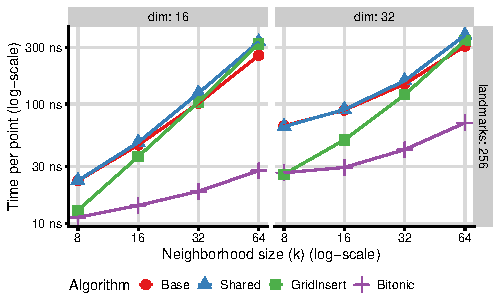
\includegraphics{embedsom/final-plots/algs_knn_repre_ampere.pdf}
	\caption{Amortized performance of $k$-NN step for a single input point using parameters usual in flow cytometry}
	\label{fig:knn-result-repre}
\end{figure}

A comparison of the best parametrizations of each algorithm on various configurations common in our target use cases is shown in Figure~\ref{fig:knn-result-repre}.
The \alg{Bitonic} algorithm significantly outperformed the other algorithms.
The speedup of \alg{Bitonic} over \alg{Base} was between $3\times$ to $20\times$ and usually more than $2\times$ over the second-ranking method.

The benchmarking also confirmed a rather huge scaling difference between algorithms based on divergent insertion sort and algorithms based on sub-quadratic parallelizable sorting schemes.
We conclude that despite the simplicity that might enable GPU speedups in certain situations, the insertion sort is too slow for larger values of $k$ in this case.

As an interesting result, we observed that despite following the general recommendations, the straightforward use of shared memory (in the \alg{Shared} algorithm) did not improve overall performance over the \alg{Base}.
Quite conversely, the overhead of explicit caching even caused a slight decrease in the overall performance.

% \begin{figure}
% 	\centering
% 	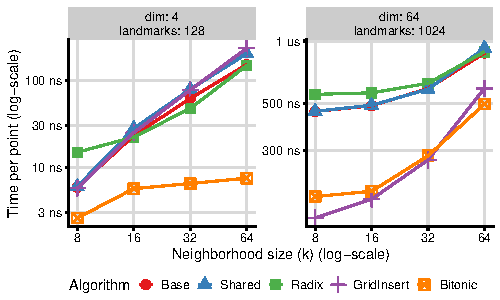
\includegraphics{embedsom/final-plots/algs_knn_extreme_ampere.pdf}
% 	\caption{Amortized $k$-NN step performance in corner-case parametrizations}
% 	\label{fig:knn-result-extreme}
% \end{figure}

We additionally report the performance measurements for two selected corner cases with extreme values of $g$ and $d$ (figure omitted due to the page limit).
Mainly, the total volume of the computation required to prepare the Euclidean distances scales with $g\cdot d$, which becomes dominant when both are maximized.
At that point, we observed that \alg{GridInsert} provides comparable or mildly better performance than \alg{Bitonic}, especially in cases where $k$ is small and the overhead of insertion sorting is not as pronounced.

Naturally, we should ask whether it could be feasible to combine the benchmarked benefits of \alg{GridInsert} and \alg{Bitonic} algorithms in order to get the best of both approaches (optimal inputs caching and fast $k$-NN filtering).
While an investigation of this possibility could be intriguing, we observed that a fused algorithm would require very complicated management of the shared memory (which both algorithms utilize heavily), and the estimated improvement of performance was not sufficient to substantiate this overhead; we thus left the question open for future research.


\subsection{Performance of projection step}

% \begin{figure}
% 	\centering
% 	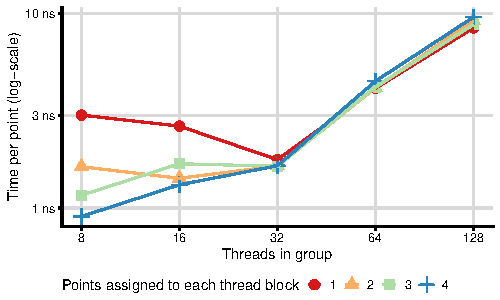
\includegraphics{embedsom/final-plots/proj_multi_block_ampere}
% 	\caption{Comparison of various sizes and numbers of thread groups in the \alg{Shared} projection algorithm in the extreme parametrization ($k = 8, d = 4$).}
% 	\label{fig:multi_block}
% \end{figure}

\begin{figure}
	\centering
	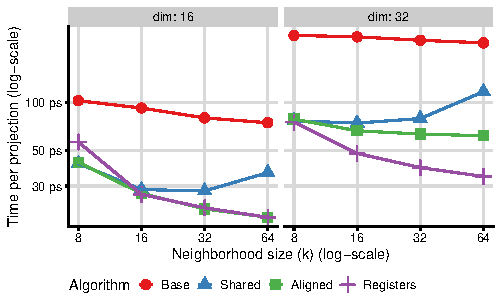
\includegraphics{embedsom/final-plots/algs_proj_repre_ampere}
	\caption{Amortized performance of a single projection operation in the algorithms that compute the projection step (showing the most important problem parametrizations)}
	\label{fig:proj_repre}
\end{figure}

The projection algorithms described in the previous section have only two execution parameters:
The size of the CUDA thread block and the number of data points assigned to a thread block (threads are divided among the points evenly).
We observed that selecting more than one point per thread block is beneficial only in the case of relatively small problem instances (low $k$ and $d$) because it prevents underutilization of the cores.

The optimal size of the CUDA thread blocks depends mainly on the parameters $k$ and $d$.
In case of \alg{Shared} algorithm, optimal values ranged from $32$ (for $k=8$, $d=4$) to $64$ ($k=d=64$).
With the caching optimizations in \alg{Aligned} and \alg{Registers}, the optimal thread block size was slightly higher, reaching $128$ for the most complex problem instances.
We assume this is a direct consequence of the improved memory access efficiency which gives space for parallel execution of additional arithmetic operations.

Figure~\ref{fig:proj_repre} shows the performance of the best algorithm configurations for the representative parametrizations.
All three algorithms perform almost equally for small $k$, giving around $3\times$ speedup over \alg{Base}.
The importance of optimizations in \alg{Aligned} and \alg{Registers} grows steadily when parameter $k$ increases, up to around $10\times$ speedup at $k=64$.
In conclusion, the optimal algorithm for the EmbedSOM projection is determined by the dimensionality of the dataset --- \alg{Registers} performs better at higher dimensions ($d\geq32$) while \alg{Aligned} was slightly better for lower dimensions.


\subsection{Complete algorithm}\label{sec:impl-complete}

A complete GPU implementation of the EmbedSOM algorithm is the combination of the best implementations of $k$-NN and projection steps.
The selected algorithms \alg{Bitonic} and \alg{Registers} are simply executed sequentially on large blocks of $X$, sharing only a single data exchange buffer for transferring the $k$-NN data.
Notably, since the data exchange between the algorithm parts is minimal, comprising only distances and neighbor indexes from the $k$-NN selection, we claim that no specific optimizations of the interface are required.

% Because of the relative complexity of the methods, we did not attempt to compute a theoretically possible data processing throughput.
% On the other hand, the collected results seem to scale proportionately to the asymptotic time complexities of the algorithms, roughly following $\mathcal{O}(n\cdot d\cdot g\cdot \log_2 k)$ for the $k$-NN and $\mathcal{O}(n\cdot d \cdot k^2)$ for the projection.
% That gives an optimistic outlook on the future scalability of the implementation, especially because the larger problem instances bear no additional overhead.

\begin{figure}
	\centering
	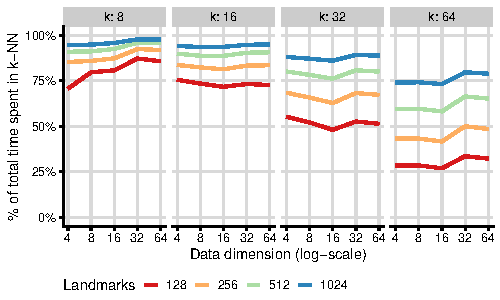
\includegraphics{embedsom/final-plots/esom_percent_ampere}
	\caption{The relative time spent by the $k$-NN computation usually dominates the execution of GPU EmbedSOM, composed of \alg{Bitonic}+\alg{Registers} algorithms.
  Projection computation time becomes dominant only for relatively impractical parametrizations of low $g$ and high $k$.}
	\label{fig:proj_percent}
\end{figure}

Finally, we highlight the relative computation complexity of both steps (Figure~\ref{fig:proj_percent}), which changes dynamically with $k$ and might be viable as a guide for further optimization.
We observed that for common parametrizations ($k\simeq 20$, $g\simeq 500$), most of the computation time is spent in $k$-NN step, and projection performance becomes problematic only in cases of almost impractically high $k$.
The results align with the asymptotic time complexities of the algorithms, roughly following $\mathcal{O}(n\cdot d\cdot g\cdot \log_2 k)$ for the $k$-NN and $\mathcal{O}(n\cdot d \cdot k^2)$ for the projection.

% The performance might be further improved by spatial indexing methods or approximate neighborhood selection algorithms, but we are currently not aware of a scheme that could provide a decisive performance improvement over the optimized brute-force neighbor processing~\cite{krulis2020detailed}.
